\documentclass[12pt]{article}
\usepackage[polish]{babel}
\usepackage[T1]{fontenc}
\usepackage{graphicx}
\usepackage{float}
\usepackage{amssymb}
\usepackage{hyperref}
\usepackage{minted}
\usepackage{fancyvrb} 

\title{Specyfikacja}
\author{Kinga Florek, Jakub Popielarz, \\Radosław Mikołajczyk}


\begin{document}

\makeatletter
    \begin{titlepage}
        \begin{center}
            
\includegraphics[scale=0.8]{agh_znk_wbr_rgb_150ppi.jpg}\\ \bigbreak
            {\Huge \bfseries  \@title }\\[2ex] 
            {\large Autorzy: \\ \@author}\\ \bigbreak
            {\large Temat projektu: \\ Orgzly synchronizacja} \\ \bigbreak
            \vspace{8mm}
            {\huge Studio Projektowe 1} \\ \bigbreak
            {\large Wydział Elektrotechniki, Automatyki, Informatyki i Inżynierii Biomedycznej} \\ 
        \end{center}
    \end{titlepage}
\makeatother



\tableofcontents
\newpage

\section{Cel projektu}

Projekt ma za zadanie roszerzyć istniejące funkcjonalności aplikacji Orgzly, która służy do notowania w formacie org-mode. Celem naszego projektu jest dodanie możliwości synchronizacji plików poprzez wykorzystanie protokołu SSH. 

\section{Identyfikacja i opis wymagań}
Wymagania, które powinno realizować oprogramowanie:
\begin{itemize}
    \item użytkownik powinien mieć możliwość wyboru synchronizacji poprzez SSH w momencie kliknięcia odpowiedniego przycisku w menu synchronizacji.
    \item po wyborze metody synchronizacji plików, aplikacja powinna wyświetlać menu logowania.
    \item menu logowania dla metody synchronizacji poprzez SSH ma umożliwiać wprowadzenie adresu serwera, nazwy użytkownika oraz hasła.
    \item dodatkowo, menu logowania powinno posiadać przycisk umożliwiający wgranie klucza SSH, którym będzie można się zalogować.
    \item aplikacja powinna obsługiwać błędy podczas logowania; powinnien zostać wyświetlony odpowiedni komunikat w zależności od błędu.
    \item użytkownik po utworzeniu nowej notatki poprzez kliknięcie przycisku w menu ma mieć możliwość umieszczania pliku na serwerze (przycisk synchronizacji na serwer).
    \item w momencie kliknięcia przycisku synchronizacji z serwera, pliki powinny być pobrane oraz zapisane w pamięci urządzenia.
    \item synchronizacja plików odbywa się przy pomocy protokołu SSH.
    \item menu Repositories zawiera dodatkową opcję SSH Connection.
\end{itemize}

\section{Design}
%Zdjecia apki gotowej itd
%dodam tu opisy jutro jak cos i poprawie to, nw czemu cos sie psuje jak nie ma \newpage
\centering{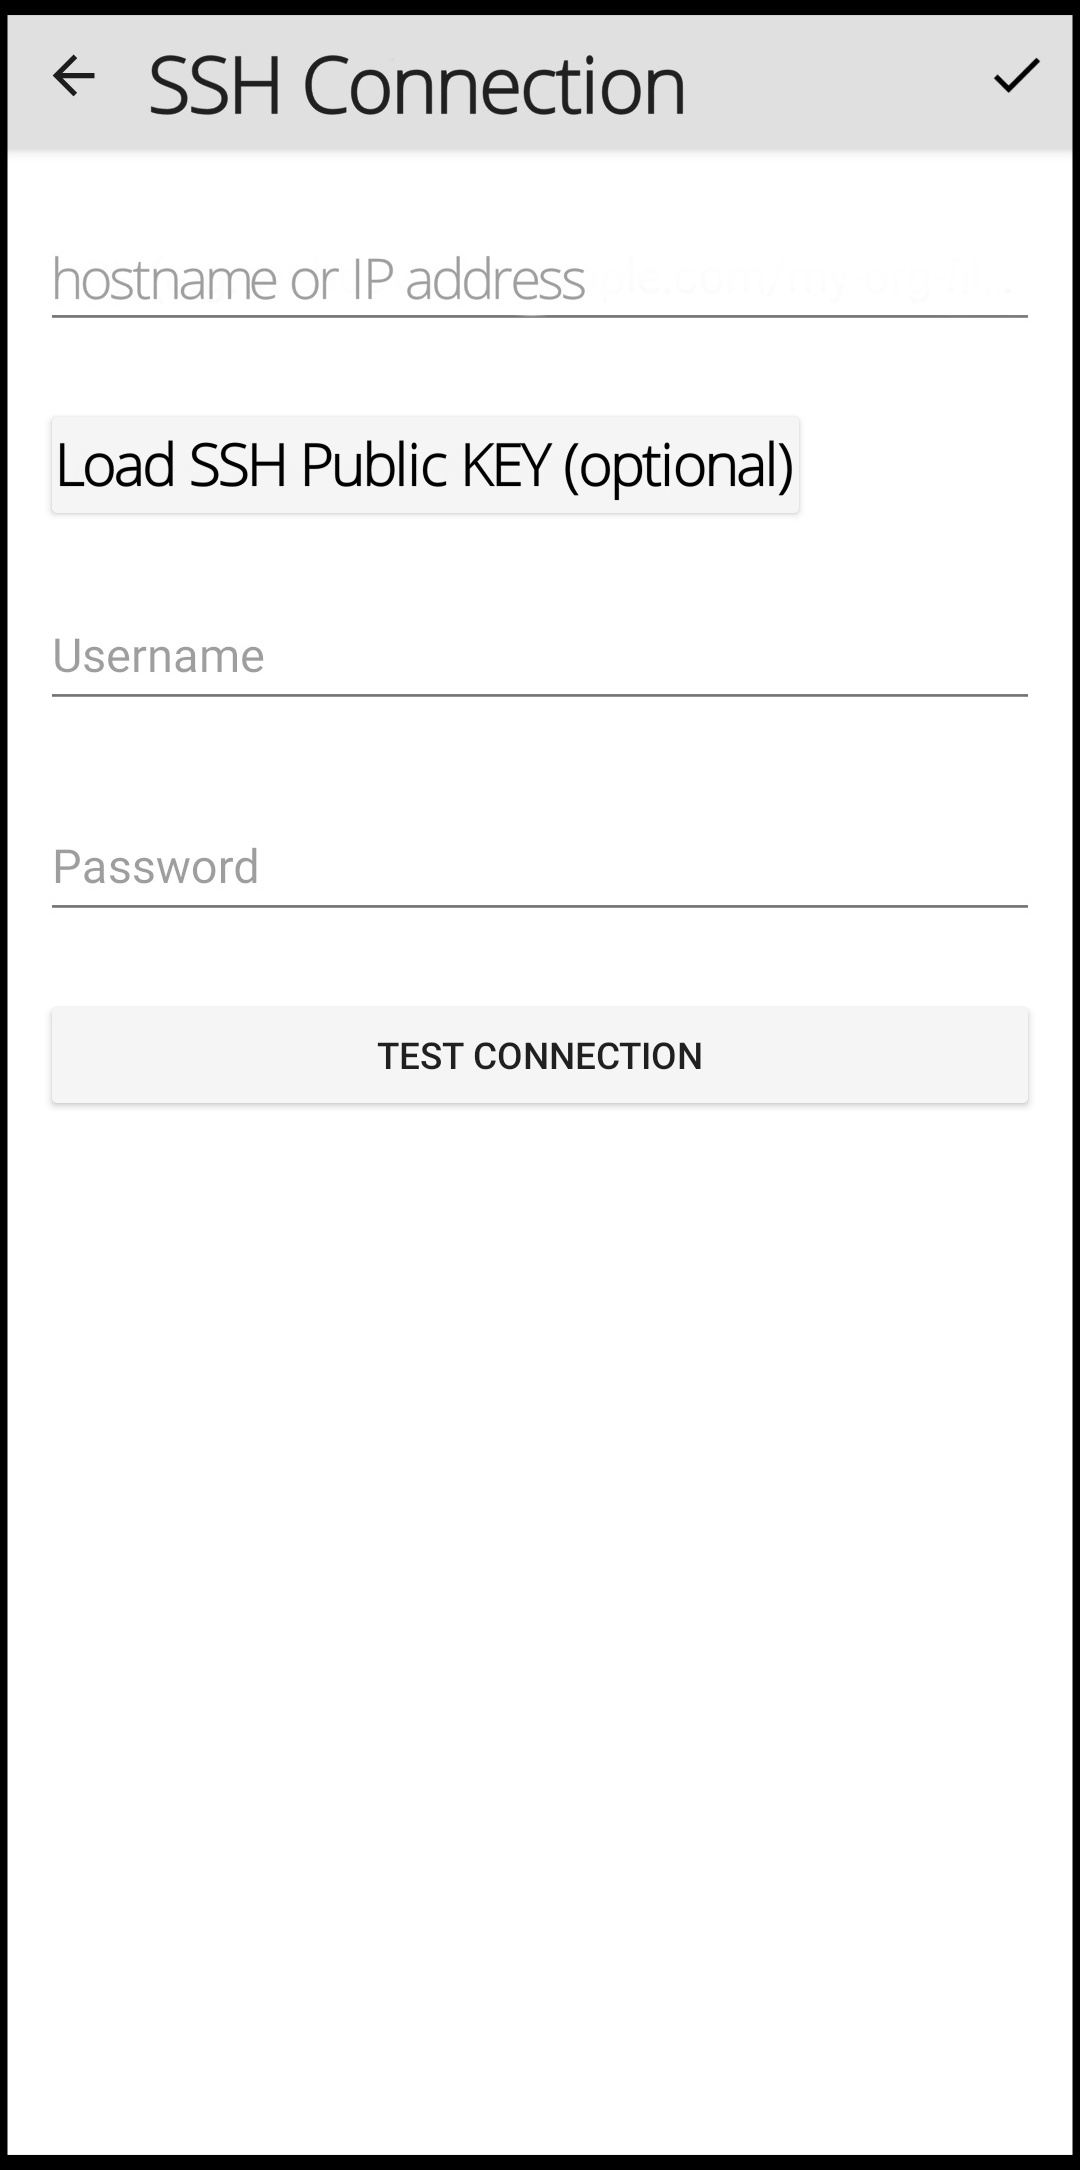
\includegraphics[scale=0.26]{2.jpg} \\
Zdjęcie poglądowe ekranu połączenia się z SSH} \\
\centering{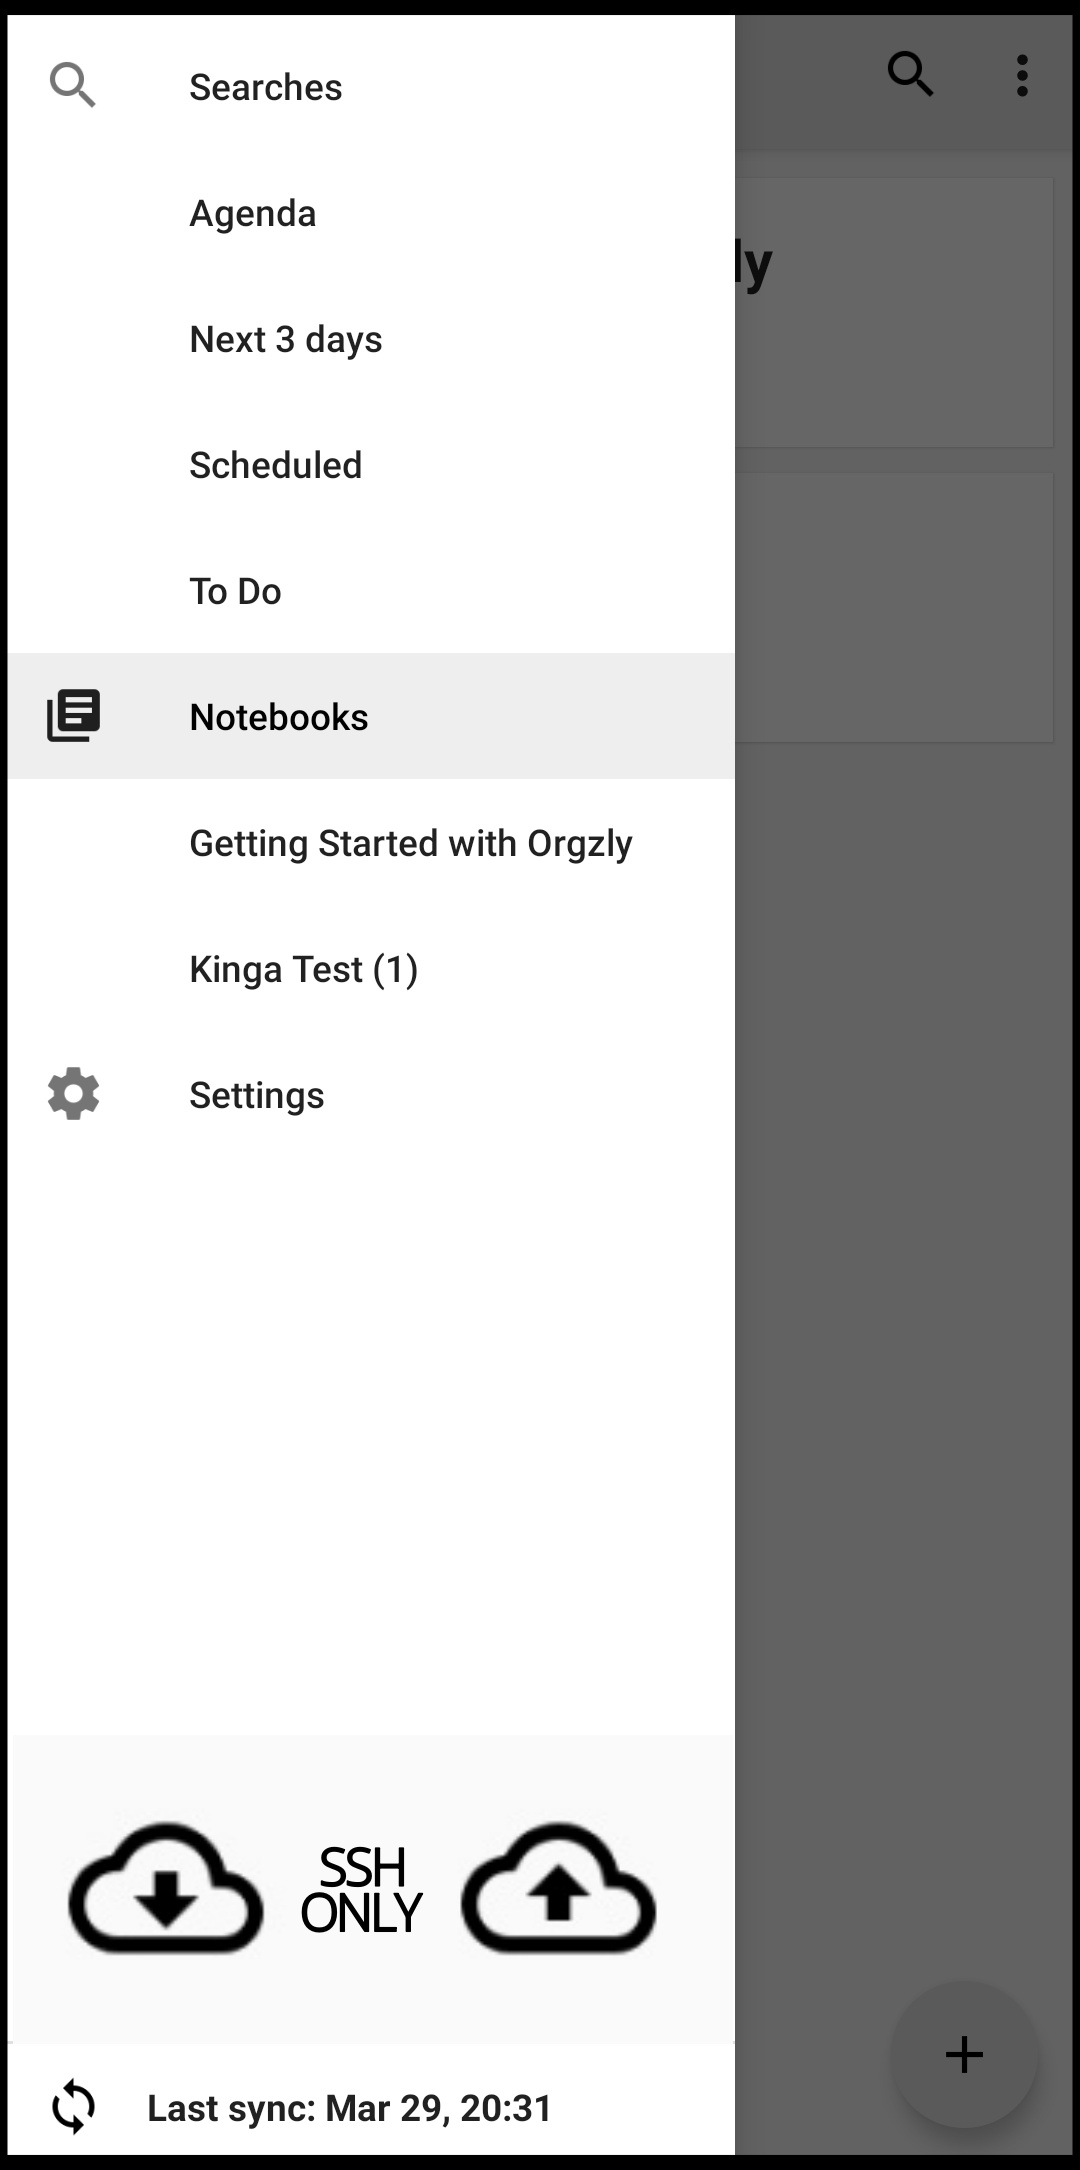
\includegraphics[scale=0.3]{3.jpg} \\
Zdjęcie poglądowe menu, w którym znajdą się przyciski pozwalające na synchronizację plików między serwerem a aplikacją}\\
\newpage
\centering{ 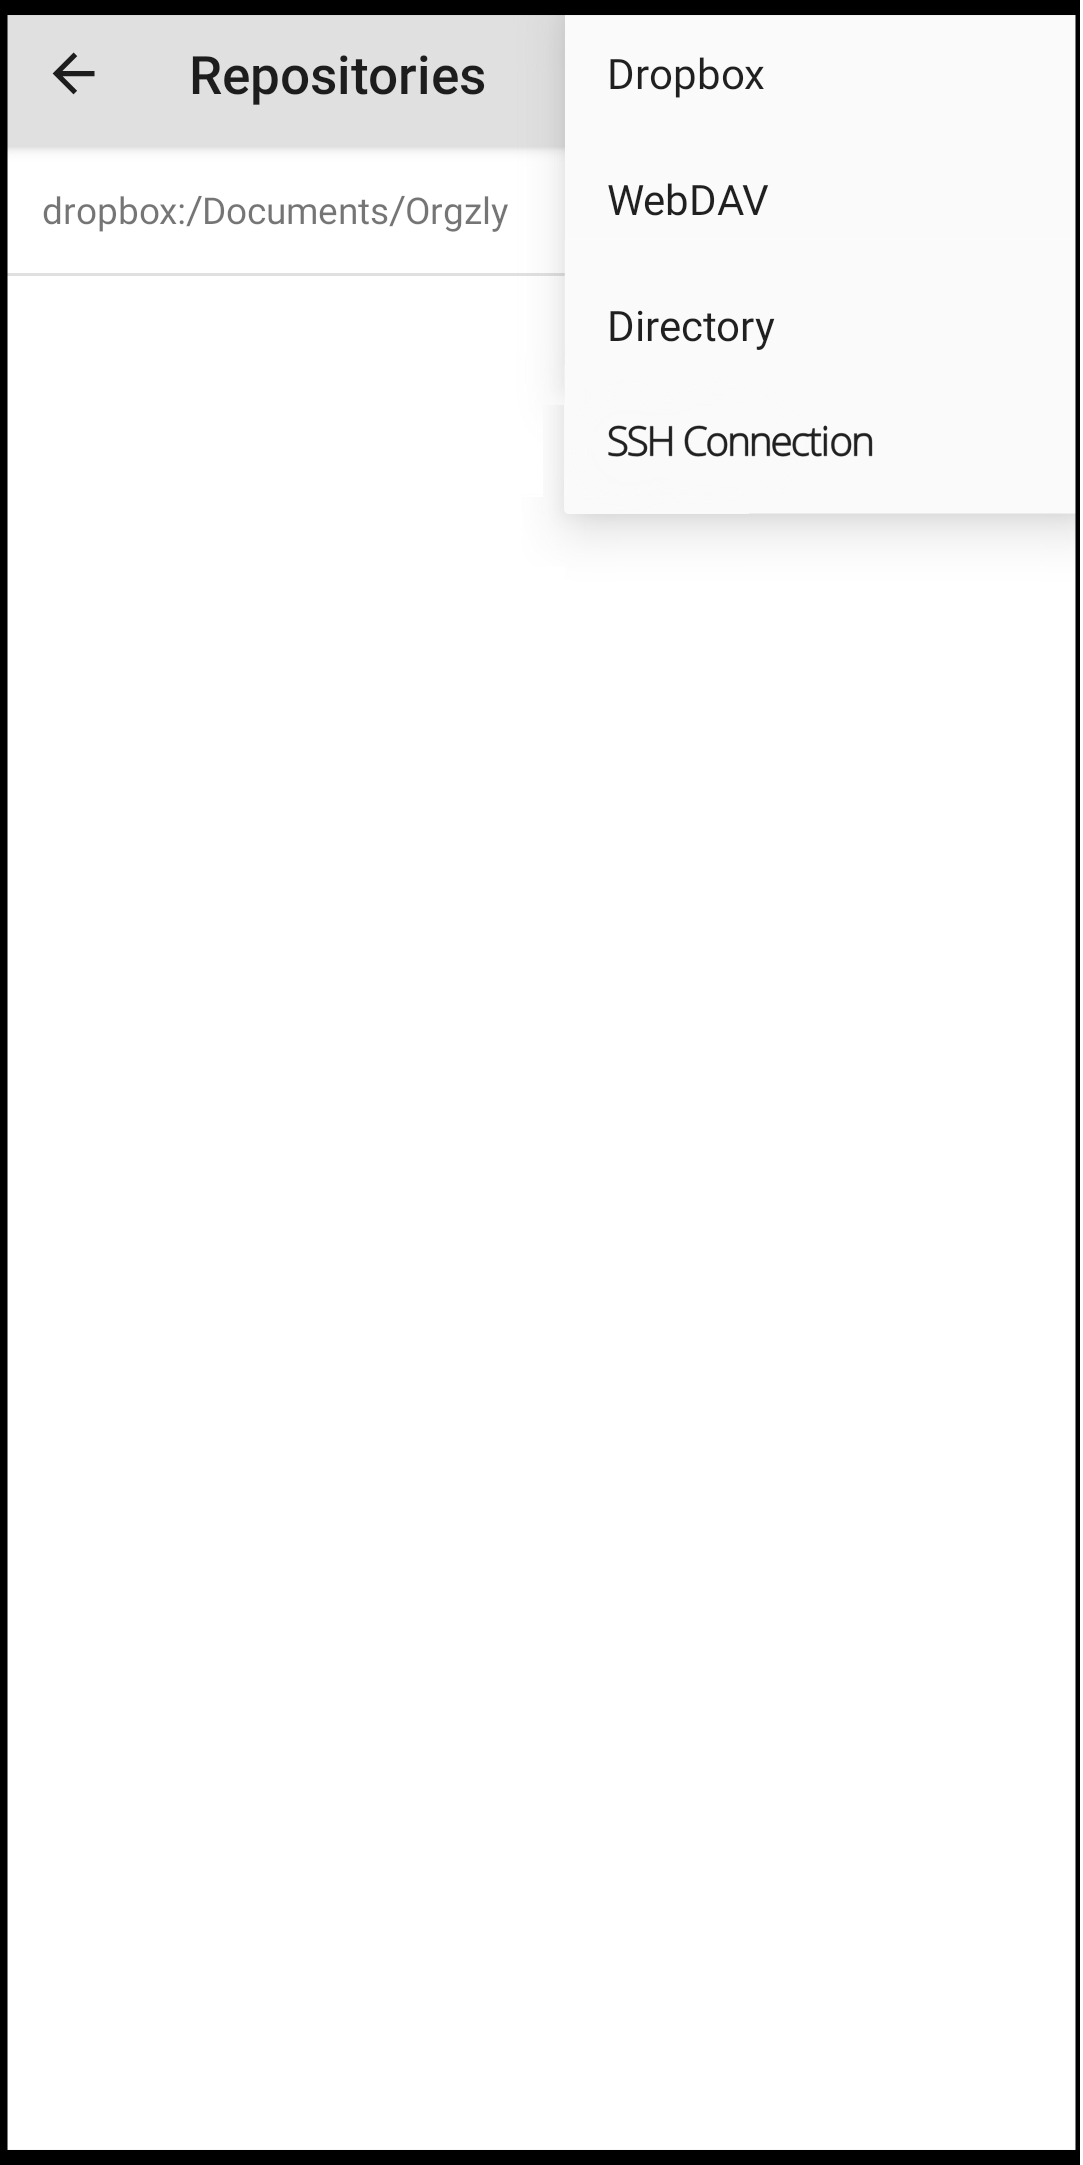
\includegraphics[scale=0.91]{1.png} \\ 
Zdjęcie poglądowe menu Repositories, w którym zostanie dodana opcja SSH Connection}
\end{document}
